\documentclass[a4paper,10pt]{book}

%%%%%%%%%%%%%%%%%%%%%%%%%%%%%%%%%%%%%%%%%
% Template Lezioni week by week
% Autore: Teo Bucci
%%%%%%%%%%%%%%%%%%%%%%%%%%%%%%%%%%%%%%%%%

%---------------------------
% FONTS AND LANGUAGE
%---------------------------

\usepackage[T1]{fontenc}
\usepackage[utf8]{inputenc}
\usepackage[english]{babel}

%---------------------------
% PACKAGES
%---------------------------

\usepackage{dsfont} % for using \mathds{1} characteristic function
\usepackage{amsmath, amssymb, amsthm} % amssymb also loads amsfonts
\usepackage{latexsym}

\usepackage{booktabs}
\usepackage{pgfplots}
\usepackage{tikz}
\usetikzlibrary{
  positioning,
  shapes.misc,
  intersections,
  shapes.symbols,
  patterns,
  fadings,
  shadows.blur,
  decorations.pathreplacing
}
\usepackage{mathdots}
\usepackage{bm}
\usepackage{cancel}
\usepackage{color}
\usepackage{siunitx}
\usepackage{array}
\usepackage{multirow}
\usepackage{makecell}
\usepackage{tabularx}
\usepackage{caption}
\captionsetup{belowskip=12pt,aboveskip=4pt}
\usepackage{subcaption}
\usepackage{placeins} % \FloatBarrier
\usepackage{flafter}  % The flafter package ensures that floats don't appear until after they appear in the code.
\usepackage[shortlabels]{enumitem}
\usepackage[italian]{varioref}
\renewcommand{\ref}{\vref}
\usepackage{hyperref}

%---------------------------
% INCLUSIONE FIGURE
%---------------------------

\usepackage{import}
\usepackage{pdfpages}
\usepackage{transparent}
\usepackage{xcolor,colortbl}
\usepackage{graphicx}
\graphicspath{ {./images/} } % Path relative to the main .tex file
\usepackage{float}

\newcommand{\fg}[3][\relax]{%
  \begin{figure}[H]%[htp]%
    \centering
    \captionsetup{width=0.7\textwidth}
      \includegraphics[width = #2\textwidth]{#3}%
      \ifx\relax#1\else\caption{#1}\fi
      \label{#3}
  \end{figure}%
  \FloatBarrier%
}
%\usepackage[labelformat=empty]{caption}


\newcommand{\quadretti}[3]{ 
\begin{tikzpicture}
\tikzset{normal lines/.style={gray, very thin}} 
\draw[style=normal lines,step=#1] (0,0) grid +(#2,#3); 
\end{tikzpicture}}

%---------------------------
% PARAGRAPHS AND LINES
%---------------------------

\usepackage[none]{hyphenat} % no hyphenation

\emergencystretch 3em % to prevent the text from going beyond margins

\usepackage[skip=0.2\baselineskip+2pt]{parskip}

% \renewcommand{\baselinestretch}{1.5} % line spacing

%---------------------------
% HEADERS AND FOOTERS
%---------------------------

\usepackage{fancyhdr}

\fancypagestyle{toc}{%
\fancyhf{}%
\fancyfoot[C]{\thepage}%
\renewcommand{\headrulewidth}{0pt}%
\renewcommand{\footrulewidth}{0pt}
}

\fancypagestyle{fancy}{%
\fancyhf{}%
\fancyhead[RE]{\nouppercase{\leftmark}}%
\fancyhead[LO]{\nouppercase{\rightmark}}%
\fancyhead[LE,RO]{\thepage}%
\renewcommand{\footrulewidth}{0pt}%
\renewcommand{\headrulewidth}{0.4pt}
}

% Removes the header from odd empty pages at the end of chapters
\makeatletter
\renewcommand{\cleardoublepage}{
\clearpage\ifodd\c@page\else
\hbox{}
\vspace*{\fill}
\thispagestyle{empty}
\newpage
\fi}

%---------------------------
% CUSTOM
%---------------------------

\definecolor{bluepoli}{cmyk}{0.4,0.1,0,0.4}

\usepackage{xspace}
\newcommand{\latex}{\LaTeX\xspace}
\newcommand{\tex}{\TeX\xspace}

\newcommand{\Tau}{\mathcal{T}}
\newcommand{\Ind}{\mathds{1}} % indicatrice

\newcommand{\transpose}{^{\mathrm{T}}}
\newcommand{\complementary}{^{\mathrm{C}}} % alternative ^{\mathrm{C}} ^{\mathrm{c}} ^{\mathsf{c}}
\newcommand{\degree}{^\circ\text{C}} % simbolo gradi

\newcommand{\notimplies}{\mathrel{{\ooalign{\hidewidth$\not\phantom{=}$\hidewidth\cr$\implies$}}}}
\newcommand{\questeq}{\overset{?}{=}} % è vero che?

\newcommand{\indep}{\perp \!\!\! \perp} % indipendenza
\newcommand{\iid}{\stackrel{\mathrm{iid}}{\sim}}
\newcommand{\event}[1]{\emph{``#1''}} % evento

% variazioni del simbolo "="
\newcommand{\iideq}{\overset{\text{\tiny iid}}{=}}
\newcommand{\ideq}{\overset{\text{\tiny id}}{=}}
\newcommand{\indepeq}{\overset{\perp \!\!\! \perp}{=}}

\newcommand{\boxedText}[1]{\noindent\fbox{\parbox{\textwidth}{#1}}}

\renewcommand{\emptyset}{\varnothing}
\renewcommand{\tilde}{\widetilde}
\renewcommand{\hat}{\widehat}

\DeclareMathOperator{\sgn}{sgn}
\DeclareMathOperator{\Var}{Var}
\DeclareMathOperator{\Cov}{Cov}
\DeclareMathOperator*{\rank}{rank}
\DeclareMathOperator*{\eig}{eig}
\DeclareMathOperator{\tr}{tr}
%\DeclareMathOperator{\Grad}{grad}
%\DeclareMathOperator{\Div}{div}
\DeclareMathOperator{\Span}{span}
\let\Re\undefined  % redefine \Re
\DeclareMathOperator{\Re}{Re}
\let\Im\undefined  % redefine \Im
\DeclareMathOperator{\Im}{Im}
\DeclareMathOperator{\Ker}{Ker}
\DeclareMathOperator*{\argmin}{arg\,min}
\DeclareMathOperator*{\argmax}{arg\,max}
\DeclareMathOperator*{\esssup}{ess\ sup}
\DeclareMathOperator*{\essinf}{ess\ inf}
\DeclareMathOperator*{\supp}{supp}

\newcommand{\eps}{\varepsilon}
\renewcommand{\theta}{\vartheta}

% Per scrivere il numero e la data della lezione


\usepackage{mathtools} % Serve per i comandi dopo
\DeclarePairedDelimiter{\abs}{\lvert}{\rvert} % absolute value
\DeclarePairedDelimiter{\norm}{\lVert}{\rVert} % norm
\DeclarePairedDelimiter{\sca}{\langle}{\rangle} % scalar product

% Bold
\renewcommand{\AA}{\mathbb A}
\newcommand{\BB}{\mathbb{B}}
\newcommand{\CC}{\mathbb{C}}
\newcommand{\DD}{\mathbb{D}}
\newcommand{\EE}{\mathbb{E}}
\newcommand{\FF}{\mathbb{F}}
\newcommand{\GG}{\mathbb{G}}
\newcommand{\HH}{\mathbb{H}}
\newcommand{\II}{\mathbb{I}}
\newcommand{\JJ}{\mathbb{J}}
\newcommand{\KK}{\mathbb{K}}
\newcommand{\LL}{\mathbb{L}}
\newcommand{\MM}{\mathbb{M}}
\newcommand{\NN}{\mathbb{N}}
\newcommand{\OO}{\mathbb{O}}
\newcommand{\PP}{\mathbb{P}}
\newcommand{\QQ}{\mathbb{Q}}
\newcommand{\RR}{\mathbb{R}}
\renewcommand{\SS}{\mathbb S}
\newcommand{\TT}{\mathbb{T}}
\newcommand{\UU}{\mathbb{U}}
\newcommand{\VV}{\mathbb{V}}
\newcommand{\WW}{\mathbb{W}}
\newcommand{\XX}{\mathbb{X}}
\newcommand{\YY}{\mathbb{Y}}
\newcommand{\ZZ}{\mathbb{Z}}

% Calligraphic
\newcommand{\Ac}{\mathcal{A}}
\newcommand{\Bc}{\mathcal{B}}
\newcommand{\Cc}{\mathcal{C}}
\newcommand{\Dc}{\mathcal{D}}
\newcommand{\Ec}{\mathcal{E}}
\newcommand{\Fc}{\mathcal{F}}
\newcommand{\Gc}{\mathcal{G}}
\newcommand{\Hc}{\mathcal{H}}
\newcommand{\Ic}{\mathcal{I}}
\newcommand{\Jc}{\mathcal{J}}
\newcommand{\Kc}{\mathcal{K}}
\newcommand{\Lc}{\mathcal{L}}
\newcommand{\Mc}{\mathcal{M}}
\newcommand{\Nc}{\mathcal{N}}
\newcommand{\Oc}{\mathcal{O}}
\newcommand{\Pc}{\mathcal{P}}
\newcommand{\Qc}{\mathcal{Q}}
\newcommand{\Rc}{\mathcal{R}}
\newcommand{\Sc}{\mathcal{S}}
\newcommand{\Tc}{\mathcal{T}}
\newcommand{\Uc}{\mathcal{U}}
\newcommand{\Vc}{\mathcal{V}}
\newcommand{\Wc}{\mathcal{W}}
\newcommand{\Xc}{\mathcal{X}}
\newcommand{\Yc}{\mathcal{Y}}
\newcommand{\Zc}{\mathcal{Z}}

% differenziale
\newcommand{\dspace}{\ } % \, aggiunge un piccolo spazio
\newcommand{\de}{\mathrm{d}}
\newcommand{\dx}{\dspace \de x}
\newcommand{\dy}{\dspace \de y}
\newcommand{\dt}{\dspace \de t}
\newcommand{\ds}{\dspace \de s}
\newcommand{\dz}{\dspace \de z}
\newcommand{\dw}{\dspace \de w}
\newcommand{\du}{\dspace \de u}
\newcommand{\dv}{\dspace \de v}
\newcommand{\db}{\dspace \de b}
\newcommand{\dteta}{\dspace \de \vartheta}
\newcommand{\dxy}{\dspace \de x \de y}
\newcommand{\duv}{\dspace \de u \de v}
\newcommand{\dst}{\dspace \de s \de t}
\newcommand{\dP}{\dspace \de P}
\newcommand{\dPP}{\dspace \de \PP}
\newcommand{\dsig}{\dspace \de \sigma}
\newcommand{\dxv}{\dspace \de \mathbf{x}}

\newcommand{\xv}{\mathbf{x}}
\newcommand{\yv}{\mathbf{y}}
\newcommand{\Fv}{\mathbf{F}}
\newcommand{\Gv}{\mathbf{G}}
\newcommand{\Grad}{\nabla}
\newcommand{\Div}{\mathrm{div}}
\newcommand{\Lap}{\Delta}
% \newcommand{\Dalem}{\Box} per l'eq delle onde?

\newcommand{\SDP}{(\Omega,\Ac,\PP)} % spazio di probabilità
\newcommand{\Omegaa}{\overline{\Omega}} % chiusura
\newcommand{\Cz}{\Cc^0}
\newcommand{\Cu}{\Cc^1}
\newcommand{\Cd}{\Cc^2}
\newcommand{\Lu}{\mathcal{L}^1}
\newcommand{\ld}{\ell^2}

%\newcommand{\Log}{\text{Log}}

% spaziature https://tex.stackexchange.com/questions/438612/space-between-exists-and-forall
% questo aggiunge un piccolo spazio dopo \forall
\let\oldforall\forall
\renewcommand{\forall}{\oldforall \, }
% questo aggiunge un piccolo spazio dopo \exists
\let\oldexist\exists
\renewcommand{\exists}{\oldexist \: }
% questo aggiunge un comando \existsu per l'esiste ed è unico
\newcommand\existu{\oldexist! \: }

%---------------------------
% APPENDICE
%---------------------------

\usepackage[title,titletoc]{appendix}

%---------------------------
% THEOREMS
%---------------------------

\definecolor{grey245}{RGB}{245,245,245}

\newtheoremstyle{blacknumbox} % Theorem style name
{0pt}% Space above
{0pt}% Space below
{\normalfont}% Body font
{}% Indent amount
{\bf\scshape}% Theorem head font --- {\small\bf}
{.\;}% Punctuation after theorem head
{0.25em}% Space after theorem head
{\small\thmname{#1}\nobreakspace\thmnumber{\@ifnotempty{#1}{}\@upn{#2}}% Theorem text (e.g. Theorem 2.1)
%{\small\thmname{#1}% Theorem text (e.g. Theorem)
\thmnote{\nobreakspace\the\thm@notefont\normalfont\bfseries---\nobreakspace#3}}% Optional theorem note

\newtheoremstyle{unnumbered} % Theorem style name
{0pt}% Space above
{0pt}% Space below
{\normalfont}% Body font
{}% Indent amount
{\bf\scshape}% Theorem head font --- {\small\bf}
{.\;}% Punctuation after theorem head
{0.25em}% Space after theorem head
{\small\thmname{#1}\thmnumber{\@ifnotempty{#1}{}\@upn{#2}}% Theorem text (e.g. Theorem 2.1)
%{\small\thmname{#1}% Theorem text (e.g. Theorem)
\thmnote{\nobreakspace\the\thm@notefont\normalfont\bfseries---\nobreakspace#3}}% Optional theorem note



\theoremstyle{blacknumbox}
\newtheorem{definitionT}{Definizione}
\newtheorem{theoremT}{Teorema}
\newtheorem{corollaryT}{Corollario}
\newtheorem{lemmaT}{Esercizio}

% Per gli unnumbered tolgo il \nobreakspace subito dopo {\small\thmname{#1} perché altrimenti c'è uno spazio tra Teorema e il ".", lo spazio lo voglio solo se sono numerati per distanziare Teorema e "(2.1)"
\theoremstyle{unnumbered}
\newtheorem*{remarkT}{Osservazione}
\newtheorem*{proofT}{Dimostrazione}
\newtheorem*{exampleT}{Esempio}

\RequirePackage[framemethod=default]{mdframed} % Required for creating the theorem, definition, exercise and corollary boxes

% orange box
\newmdenv[skipabove=7pt,
skipbelow=7pt,
rightline=false,
leftline=true,
topline=false,
bottomline=false,
linecolor=orange,
backgroundcolor=orange!0,
innerleftmargin=5pt,
innerrightmargin=5pt,
innertopmargin=5pt,
leftmargin=0cm,
rightmargin=0cm,
linewidth=2pt,
innerbottommargin=5pt]{oBox}

% green box
\newmdenv[skipabove=7pt,
skipbelow=7pt,
rightline=false,
leftline=true,
topline=false,
bottomline=false,
linecolor=green,
backgroundcolor=green!0,
innerleftmargin=5pt,
innerrightmargin=5pt,
innertopmargin=5pt,
leftmargin=0cm,
rightmargin=0cm,
linewidth=2pt,
innerbottommargin=5pt]{gBox}

% blue box
\newmdenv[skipabove=7pt,
skipbelow=7pt,
rightline=false,
leftline=true,
topline=false,
bottomline=false,
linecolor=blue,
backgroundcolor=blue!0,
innerleftmargin=5pt,
innerrightmargin=5pt,
innertopmargin=5pt,
leftmargin=0cm,
rightmargin=0cm,
linewidth=2pt,
innerbottommargin=5pt]{bBox}

% dim box
\newmdenv[skipabove=7pt,
skipbelow=7pt,
rightline=false,
leftline=true,
topline=false,
bottomline=false,
linecolor=black,
backgroundcolor=grey245!0,
innerleftmargin=5pt,
innerrightmargin=5pt,
innertopmargin=5pt,
leftmargin=0cm,
rightmargin=0cm,
linewidth=2pt,
innerbottommargin=5pt]{blackBox}

\newenvironment{defn}{\begin{bBox}\begin{definitionT}}{\end{definitionT}\end{bBox}}
\newenvironment{thm}{\begin{gBox}\begin{theoremT}}{\end{theoremT}\end{gBox}}
\newenvironment{coro}{\begin{oBox}\begin{corollaryT}}{\end{corollaryT}\end{oBox}}
\newenvironment{es}{\begin{bBox}\begin{lemmaT}}{\end{lemmaT}\end{bBox}}
\newenvironment{rem}{\begin{oBox}\begin{remarkT}}{\end{remarkT}\end{oBox}}
\newenvironment{exa}{\begin{blackBox}\begin{exampleT}}{\end{exampleT}\end{blackBox}}

\renewcommand{\qed}{\tag*{$\blacksquare$}}
\renewenvironment{proof}{\begin{blackBox}\begin{proofT}}{\[\qed\]\end{proofT}\end{blackBox}}

% ==========================================================

\RequirePackage{verbatim}
\RequirePackage{fancyvrb}
\RequirePackage{color}

\newcommand{\maxwidth}[1]{\ifdim\linewidth>#1 #1\else\linewidth\fi}
\newcommand{\mlcell}[1]{{\color{output}\verbatim@font#1}}

\definecolor{output}{gray}{0.4}

% Unicode character conversions
\DeclareUnicodeCharacter{B0}{\ensuremath{^\circ}}
\DeclareUnicodeCharacter{21B5}{\ensuremath{\hookleftarrow}}

\newenvironment{matlaboutput}{%
        \Verbatim[xleftmargin=1.25em, formatcom=\color{output}]%
}{\endVerbatim}

\usepackage[
    left=2.5cm, % inner
    right=2.5cm, % outer
    top=1.5cm,
    bottom=1.5cm,
    %showframe,
    ]{geometry}

\usepackage{titling}
\newcommand{\subtitle}[1]{%
  \posttitle{%
    \par\end{center}
    \begin{center}\large#1\end{center}
    \vskip0.5em}%
}

\usepackage{listings}

\lstset{
    language=C++,
    %alsolanguage=[ANSI]C,
    basicstyle=\small\ttfamily,
    numbers=none,
    numberstyle=\tiny,
    stepnumber=1,
    frame=single
}

\lstset{
    literate=
        {è}{{\ttfamily\`e}}1
        {à}{{\ttfamily\`a}}1
        {ì}{{\ttfamily\`i}}1
        {ò}{{\ttfamily\`o}}1
        {ù}{{\ttfamily\`u}}1
        {-}{{\ttfamily -}}1
        {\&}{{\sffamily \&}}1
        {<}{{\sffamily <}}1
        {>}{{\sffamily >}}1,
    % language=C++,
    keywordstyle=\color{red}, 
    keywordstyle=[2]{\color{purple}},
    directivestyle=\color{red},
    commentstyle=\color{blue},
    stringstyle=\color{teal},
    % basicstyle=\small\ttfamily,
    showstringspaces=lines,
    keepspaces,
    % tabsize=4,
    deletekeywords={operator, string, char},
    morekeywords={include, size_t, ifndef, define},
    morekeywords=[2]{main},
    otherkeywords={\#},
    %moredelim=*[directive]\#,
    %moredirectives={main},
}
%deletekeywords={}, morekeywords={}, rulecolor=\color{blue}

\usepackage[most]{tcolorbox}

\newtcolorbox{marker}[1][]{enhanced,
    before skip=2mm,after skip=5mm,
    boxrule=0.4pt,left=5mm,right=2mm,top=1mm,bottom=1mm,
    colback=yellow!50,
    colframe=yellow!20!black,
    sharp corners,rounded corners=southeast,arc is angular,arc=3mm,
    underlay={%
        \path[fill=tcbcolback!80!black] ([yshift=3mm]interior.south east)--++(-0.4,-0.1)--++(0.1,-0.2);
        \path[draw=tcbcolframe,shorten <=-0.05mm,shorten >=-0.05mm] ([yshift=3mm]interior.south east)--++(-0.4,-0.1)--++(0.1,-0.2);
        \path[fill=yellow!50!black,draw=none] (interior.south west) rectangle node[white,rotate=0]{\Huge\bfseries ! } ([xshift=4mm]interior.north west);
    },
    drop fuzzy shadow,#1}

\newcommand*\circled[1]{\tikz[baseline=(char.base)]{
    \node[shape=circle,draw,inner sep=2pt] (char) {#1};}}


\usepackage{pdfpages}
\includepdfset{pages=-, frame, offset=0mm 1cm,
   pagecommand={\thispagestyle{empty}}}

\newcommand*{\TakeFourierOrnament}[1]{{%
\fontencoding{U}\fontfamily{futs}\selectfont\char#1}}
\newcommand*{\danger}{\TakeFourierOrnament{49}}

\usepackage{chngcntr}
\counterwithout{figure}{chapter}
\counterwithout{figure}{section}

% =================================================================

\begin{document}

\frontmatter

\thispagestyle{empty}
\vspace*{\fill}

\begin{center}

    \fg{0.5}{images/logo_polimi}

    \vspace*{3cm}

    {\large Labs of}\\
    
    \vspace*{1.5cm}
    
    {\Huge \textsc{NLA}}\\
    
    \vspace*{1.5cm}
    
    {\large taught by Professor Paola Antonietti}\\
    \vspace*{0.3cm}
    {\large Master Degree in Mathematical Engineering, Polimi, 2024/25}\\

    \vspace*{6cm}

    {\large By}\\
    \vspace*{0.3cm}
    {\large Teo Bonfa}\\

    \vspace*{1.5cm}

    \fg{0.2}{images/logo_blackCL}
\end{center}
\vspace*{\fill}
\clearpage

% INDICE

\cleardoublepage
\tableofcontents
\cleardoublepage

\mainmatter
\pagestyle{empty}

%!TEX root = ../main.tex

\chapter{Classes-1}
\thispagestyle{empty}

In C++ we use classes to define our own \textbf{abstract data types} (ADT). By defining types that mirror concepts in the problems we are trying to solve, we can make our programs easier to write,
debug, and modify.

\section{Classes basics} % (fold)
\label{sec:classes_basics}

\begin{itemize}[$\triangleright$]
\item Classes are user-defined type, i.e. specifies a blueprint for objects.

\begin{marker}
    Most fundamentally, a class defines a new type and a new scope.
\end{marker}

\item Each class consists of a set of members. Members can be either data (\textbf{data members}), functions (\textbf{member functions} or \textbf{methods}), or type definitions.

\item Member functions can define the meaning of creation (constructor), initialization, assignment, copy, and cleanup (destruction).

\item A class may contain multiple \texttt{public}, \texttt{private}, and \texttt{protected} sections. Members defined in the \texttt{public} section are accessible to all code that uses the type; those defined in the \texttt{private} section are accessible (only) to other class members. We'll have more to say about \texttt{protected} when we discuss inheritance.

\begin{marker}
The public members provide the class \textbf{interface} and the private members provide \textbf{implementation details} that we want to hide.
\end{marker}

\item First example:
\begin{lstlisting}
class X { // this class' name is X

private: // private members <-- that's the implementation details 
    // (accessible by members of this class only)
    // functions
    // types
    // data

public: // public members <-- that's the interface to users
    // (accessible by all)
    // functions
    // types
    // data (often best kept private!)
};
\end{lstlisting}

\item Members are accessed using . (dot) for objects and -> (arrow) or (* ). (dereference plus dot) for pointers:
\begin{lstlisting}
// in a header file
class Complex {
private:
    double m_real;
    double m_img;
    int mf1();
public:
    int mf2();
};

// in the main
Complex num; // object (variable) num of type Complex
Complex *ptr = &num; // pointer of type Complex to num

double re = num.m_real; // ERROR: m_real is private
int i = num.mf1(); // ERROR: m_real is private
int j = ptr->mf2(); // good
int k = (*ptr).mf2(); // same as previous
\end{lstlisting}

\begin{marker}
Class members are private by default. So in the example you might omit the \texttt{private} key.
\end{marker}

\item Also operators, such as +, !, and [ ], can be defined as well (e.g. what is the meaning of + between two object from the class \texttt{Complex}).
\end{itemize}

% section classes_basics (end)

\section{Classes and Struct} % (fold)
\label{sec:classes_and_struct}

A struct is a class where members are public by default. So
\begin{lstlisting}
struct X {
    int m;
};
\end{lstlisting}
is equivalent to
\begin{lstlisting}
class X {
public:
    int m;
};
\end{lstlisting}

But then:
\begin{itemize}
    \item which are the benefits of classes (i.e. public/private)?
    \item when shall we use a class and when a struct?
\end{itemize}

\bigskip

Let's answer.
\begin{enumerate}[$\triangleright$]
    \item We do not make everything public
    \begin{itemize}
        \item to provide a clean interface (data and messy functions can me hidden)

        \item to allow a change of representation (we'll se in the complex numbers example)

        \begin{marker}
        If internal representation is hidden (\textbf{information hiding} principle):
        \begin{itemize}
            \item it's easier to support code evolution
            \item we can change the internals without changing the remaining code
        \end{itemize}
        \end{marker}

        \item to make sure that sensitive members are not used/copied/modified by anyone

        \item to ease debugging

        \item to maintain an \textbf{invariant}
    \end{itemize}

    \item What are invariants? Let's consider the \texttt{Date} example. 

    To verify if the value of a date is valid (e.g. the month cannot be 13) we have to check for validity all the time, or we try to design our types so that values are guaranteed to be valid.

    A rule for what constitutes a valid value is called an \textbf{invariant}.

    The invariant for dates ("a date must represent a date in the past, present, or future") is usually hard to state precisely because of February 29th, leap years (\emph{anni bisestili}), etc.

    \begin{marker}
    If we can't thing of a good invariant, we can probably use struct.
    \end{marker}

    \newpage

    Let's implement \texttt{Date} using struct:
    \begin{lstlisting}
struct Date {
    int day, month, year;
}

int main() {
    Date my_birthday;
    my_birthday.day = 15;
    my_birthday.month = 5;
    my_birthday.year = 2000;
}
\end{lstlisting}

    We have to add a few helper functions for convenience:
    \begin{lstlisting}
void init_date(Date& date, int day, int month, int year) {
    // check for valid date and initialize ...
}

void add_day(Date& date, int n) {
    // increase date by n days ...
}
\end{lstlisting}

    Admitting for a moment a trivial invariant, we have this:
    \begin{lstlisting}
#include <iostream>

struct Date {
    int day, month, year;
};

void init_date(Date& date, int day, int month, int year);
void add_day(Date& date, int n);

int main() {
    Date my_birthday;
    init_date(my_birthday, 15, 5, 2000);
    std::cout << my_birthday.day << "/" << my_birthday.month 
              << "/" << my_birthday.year << "\n";

    Date your_birthday = my_birthday;
    add_day(your_birthday, 11);
    std::cout << your_birthday.day << "/" << your_birthday.month 
              << "/" << your_birthday.year << "\n";

    return 0;
}

void init_date(Date& date, int day, int month, int year) {
    // check for valid date and initialize ...
    if (day<=31 && month<=12) {
        date.day = day;
        date.month = month;
        date.year = year;
    }
}

void add_day(Date& date, int n) {
    // increase date by n days ...
    init_date(date, date.day + n, date.month, date.year);
}
\end{lstlisting}

    The output is the following: \lstinline|15/05/2000| and \lstinline|26/05/2000|. 

    \newpage

    \item There is a better way to  do this, using a \textbf{constructor}:
    \begin{lstlisting}
#include <iostream>

struct Date {
    int day, month, year;
    Date (int d, int m, int y) {
        if (d<=31 && m<=12) {
            day = d;
            month = m;
            year = y;
        }
    };
};

int main() {
    Date my_birthday(15, 5, 2000);
    std::cout << my_birthday.day << "/" << my_birthday.month
              << "/" << my_birthday.year << "\n";

    return 0;
}
\end{lstlisting}

    \begin{marker}
    When we create an object of a class type, the compiler automatically uses a constructor to initialize the object. A constructor is a special member function that has the same name as the class. Its purpose is to ensure that each data member is set to sensible initial values.  
    \end{marker}

    Moving on to classes, we can prevent someone from manually editing, for example, the month of a date, making it invalid.

    Let's create a class in CLion:
    \begin{enumerate}
        \item create a new project $\to$ right click on the folder name $\to$ new $\to$ C++ class
        \item insert the name of the class, our is \texttt{Date}
        \item the \texttt{Date.h} file will open
        \item write this:
        \begin{lstlisting}
#ifndef MYDATECLASS_DATE_H
#define MYDATECLASS_DATE_H

class Date {
    int d, m, y; // private by default
public:
    Date(int d, int m, int y);
    void add_day(int n);
    int month() const;
};

#endif //MYDATECLASS_DATE_H     
\end{lstlisting}
        \item right click on the file $\to$ generate $\to$ generate definitions
        \item hold Shift and click on every members $\to$ ok $\to$ the \texttt{Date.cpp} file will open:
        \begin{lstlisting}
#include "Date.h"

Date::Date(int d, int m, int y) {

}

void Date::add_day(int n) {

}

int Date::month() const {
    return 0;
}
\end{lstlisting}
        \item now go to \texttt{main.cpp}, add \lstinline|#include "Date.h"| and you can write your own main
    \end{enumerate}

    For example, you can write \lstinline|Date birthday(15,5,2000);| and the compiler will create the object \texttt{birthday} of type \texttt{Date} intialized at $15/5/2000$.

    Some important things:
    \begin{itemize}
        \item Now you can't write \lstinline|std::cout << birthday.day << "\n";| because the member \texttt{day} is private!

        \begin{marker}
        To print values of private members you have to use a print function within the class. Why? Because private members are accessible by other members of the same class! You can't access them directly, you have to go through the class!
        \end{marker}

        \item A constructor gets called automatically when we create the object of the class.

        \item There are plenty of ways to create a constructor. In this example, the constructor is
        \begin{lstlisting}
Date::Date(int d, int m, int y) {

}
\end{lstlisting}

        This is the \emph{default style}, because if you don't declare one, the compiler will automatically create a constructor like that.

        \item The name of the constructor is same as its class name.

        \item Constructors are mostly declared in the public section of the class, though they can be declared in the private section too.

        \item Constructors do not return values; hence \textbf{they do not have a return type}.

        \item Constructors can be defined inside or outside the class declaration. In this case, we have declared the constructor in a header but we have defined it in a source file. So we needed to use the \textbf{scope operator} :: ("member of") to clarify that the constructor is the constructor of the \texttt{Date} class.

        \item Member functions may be declared \texttt{const} (\lstinline|int Date::month() const|). A \texttt{const} member may not change the data members of the object on which it operates.
    \end{itemize}

    \item Another example:
    \begin{lstlisting}
class Line {
public:
    void setLength(double len); // <-- setter
    double getLength(); // <-- getter
    Line(double len); // <-- constructor
private:
    double length;
};
// member functions definition
Line::Line(double len) {
    cout<<"Object is being created, length = "<< len <<endl;
    length = len;
}
void Line::setLength(double len) {
    length = len;
}
double Line::getLength() {
    return length;
}
// main function for the program
int main() {
    Line line(10.0);
    std::cout<<"Length of line : " << line.getLength() << std::endl;
    line.setLength(6.0);
    std::cout<<"Length of line : " << line.getLength() << std::endl;
}
\end{lstlisting}

    The output is: \\
    \lstinline|Object is being created, length = 10| \\
    \lstinline|Length of line : 10| \\
    \lstinline|Length of line : 6|

    \newpage

    \item Write a class named Person that represent the name and address of a person. Provide a constructor, and some getters and setters.
    \begin{lstlisting}
// Person.h
#ifndef PERSON_PERSON_H
#define PERSON_PERSON_H

#include <string>

class Person {
    std::string name;
    std::string address;
public:
    // Constructor
    Person(std::string, std::string);
    // Setter
    void set_name(std::string);
    void set_address(std::string);
    // Getter
    std::string get_name() const;
    std::string get_address() const;
    // Print
    void print() const;
};

#endif //PERSON_PERSON_H
\end{lstlisting}
    \begin{lstlisting}
// Person.cpp
#include "Person.h"
#include <iostream>

Person::Person(std::string Name, std::string Address) {
    name = Name;
    address = Address;
}

void Person::set_name(std::string Name) {
    name = Name;
}

void Person::set_address(std::string Address) {
    address = Address;
}

std::string Person::get_name() const {
    return name;
}

std::string Person::get_address() const {
    return address;
}

void Person::print() const {
    std::cout << "Person is " << name << ", at " << address << std::endl;
}
\end{lstlisting}
    \begin{lstlisting}
// main.cpp
#include <iostream>
#include "Person.h"

int main() {
    Person you("Lorenzo", "Milano");
    you.print();
    return 0;
}
\end{lstlisting}
\end{enumerate}

% section classes_and_struct (end)

\section{The implicit \texttt{this} pointer} % (fold)
\label{sec:the_implicit_this_pointer}

Member functions have an extra implicit parameter that is a \textbf{pointer to an object of the class type}. This implicit parameter is named \texttt{this}, and it is bound to the object on which the member function is called. 

So member functions access the object on which they were called through the \texttt{this} pointer.

\begin{marker}
Member functions may not define the \texttt{this} parameter, the compiler does so implicitly. 

The body of a member function may explicitly use the \texttt{this} pointer, but is not required to do so; there are only two exception: for \texttt{static} members and when we need to refer to the object as a whole rather than to a member of the object. 
\end{marker}

Take a look at this:
\begin{lstlisting}
Date my_birthday(15, 5, 2000);
int may = my_birthday.m();
\end{lstlisting}

Here we used the dot operator to run \texttt{month()} on the object named \texttt{my\_birthday}. So the method \texttt{month()} is referring implicitly to the members of the object on which the function was called.

When we call a member function, \textbf{\texttt{this} is initialized with the address of the object on which the function was invoked}. For example, when we call \lstinline|my_birthday.m()| the compiler passes the address of \texttt{my\_birthday} to the implicit \texttt{this} parameter; then the method \texttt{month()} return \texttt{this->m}.

\fg{1}{birth.png}

This is how it works, but in reality we do not do that: the \texttt{this} parameter is defined for us implicitly.

\begin{marker}
\begin{itemize}
    \item It is illegal for us to define a parameter or variable named \texttt{this}
    \item \texttt{this} is a \textbf{const pointer}, we cannot change the address that it holds.
\end{itemize}
\end{marker}

\subsection*{\texttt{PlayWithThis} example}

Let's create a trivial class, with a constructor and a getter:
\begin{lstlisting}
// X.h
class X {
private:
    int x;
public:
    X(int x); // <-- constructor
    int get_x() const; // <-- getter
};
\end{lstlisting}
\begin{lstlisting}
// X.cpp
#include "X.h"

X::X(int x) {
    x = x;
}

int X::get_x() const {
    return x;
}
\end{lstlisting}
\begin{lstlisting}
// main.cpp
#include <iostream>
#include "X.h"

int main() {
    X obj(3);
    std::cout << obj.get_x() << std::endl;
    return 0;
}
\end{lstlisting}

Rather than the expected 3 output, we get a different value every time we run the code. This occurrence of random values is typical in situations where the variable is not initialized.

So where’s the mistake here?

Surely, it's in the constructor. Because of \textbf{variable scope}, when we said \texttt{x=x} we were actually doing a self-assignment with the function input \texttt{x}, we're not touching the class member \texttt{x}.

To fix the error:
\begin{lstlisting}
X::X(int x) {
    this->x = x;
}
\end{lstlisting}
because with \texttt{this} we are able to access the members of the class we're dealing.

In real life we simply use different names:
\begin{lstlisting}
X::X(int x) {
    x = xx;
}   
\end{lstlisting}

% section the_implicit_this_pointer (end)

\section{Helper functions} % (fold)
\label{sec:helper_functions}

What makes a good \textbf{class interface} (the set of public functions)?
\begin{itemize}
    \item Minimal (as small as possible)
    \item Complete (and no smaller)
    \item Invariant preserving
    \item Const correct
\end{itemize}

We keep a class interface minimal because it
\begin{itemize}[>]
    \item simplifies understanding
    \item simplifies debugging
    \item simplifies maintenance
\end{itemize}
but we need extra (non-member) "helper functions" outside the class, for example \lstinline|next_weekday| or the opeators \lstinline|==| and \lstinline|!=| to compare two dates. 

\begin{marker}
\begin{itemize}
        \item Declare helper functions in the class header
        \item Define helper functions the class source file
\end{itemize}    
\end{marker}  

% section helper_functions (end)

\newpage

\section{Operator overloading} % (fold)
\label{sec:operators}

\begin{enumerate}[$\triangleright$]
\item C++ let us redefine the meaning of the operators when applied to objects of class type.
\item Judicious use of \textbf{operator overloading} can make class types as intuitive to use as the built-in types.
\item For example, the standard library defines several overloaded operators for the container classes. These classes define the subscript operator [ ] to access data elements and * and -> to dereference container iterators. The fact that these library types have the same operators makes using them similar to using built-in arrays and pointers. Allowing programs to use expressions rather than named functions can make the programs much easier to write and read.
\item Overloaded operators are functions with special names: the keyword operator followed by the symbol for the operator being defined. Like any other function, an overloaded operator has a return type and a parameter list: \lstinline|Complex operator+(const Complex&, const Complex&);| 

\item There are some rules and some advices to follow:
\begin{enumerate}[(1)]
    \item An overloaded operator has the same number of parameters as the operator has operands (e.g., no \texttt{operator<=} with only one parameter (unary), or \texttt{operator!} (not) with two parameters (binary)), except for the function-call operator: \texttt{operator()}

    \item There are operators that may be and may not be overloaded:
    \fg{0.65}{maynot}

    \item New operators may not be created by concatenating other legal symbols (e.g., it would be illegal to attempt to define an \texttt{operator**} to provide exponentiation)

    \begin{marker}
    You can define only existing operators, you can not create new ones.
    \end{marker}

    \item The meaning of an operator for the built-in types may not be changed (e.g., the built-in integer addition operation cannot be redefined)

    Nor may additional operators be defined for the built-in data types (e.g., an \texttt{operator+} taking two operands of array types cannot be defined)

    \begin{marker}
    An overloaded operator must have at least one user-defined type as operand. This rule enforces the requirement that an overloaded operator may not redefine the meaning of the operators when applied to objects of built-in type.
    \end{marker}

    \item The precedence, associativity, or number of operands of an operator cannot be changed (e.g., regardless of the type of the operands and regardless of the definition of what the operations do, the expression \texttt{x == y+z} always binds the arguments \texttt{y} and \texttt{z} to \texttt{operator+} and uses that result as the right-hand operand to \texttt{operator==})

    \item Four symbols (+, -, * , \&) serve as both unary (with one operand) and binary (with two operands) operators, which operator is being defined is controlled by the number of operands

    \item Overload operators only with their conventional meaning (e.g., + should be addition)

    \item Don't overload \&\&, ||, and the comma operator (because the order in which those operands are evaluated is not stipulated or defined)

    \item \textbf{Don’t overload unless you really have to}
\end{enumerate}

\item Class example: \texttt{MatlabVector}

We want to implement Matlab-like vectors in C++, so vectors can grow as in Matlab 
\fg{0.6}{matv}
but we want to keep the C++ convention for elements indexing (i.e. the first element has index 0). 

So our goals are:
\begin{itemize}
    \item provide \texttt{operator+}
    \item implement the product of \texttt{MatlabVector} with a scalar: \texttt{operator*}
    \item provide \texttt{operator[]} to access individual elements
    \item neglect, in the beginning, errors (e.g., vectors size do not match)
\end{itemize}

Our first implementation is the following:
\begin{lstlisting}
class MatlabVector {

    std::vector<double> elem;

public:

    void set(size_t n, double v); // access: write
    double get(size_t n); // access: read

    size_t size() const; // return number of elements

    void print() const;

    MatlabVector operator*(double scalar) const;
};

MatlabVector operator+(MatlabVector& v1, MatlabVector& v2);   
\end{lstlisting}

Note that:
\begin{itemize}
    \item the getter is not const, beacuse if the index is out of dimension we want the automatically growth of the vector

    \item the \texttt{operator*} is const, because we're not changing the object which we're computing on

    \item the \texttt{operator+} is not in the class, it's a helper function, and so it uses references to access the members of the class (and the references are not const because the getter is not const!)
\end{itemize}

Let's see the functions in details:
\begin{lstlisting}
void MatlabVector::set(size_t n, double v)
{
    while (elem.size() < n+1)
        elem.push_back(0.);
    
    elem[n] = v;
}

double MatlabVector::get(size_t n)
{
    while (elem.size() < n+1)
        elem.push_back(0.);

    return elem[n];
}

size_t MatlabVector::size() const
{
    return elem.size();
}

MatlabVector MatlabVector::operator*(double scalar) const
{
    MatlabVector result;

    for (unsigned i=0; i<elem.size(); ++i)
        result.set(i, scalar * elem[i]);

    return result;
}

MatlabVector operator+(MatlabVector& v1, MatlabVector& v2)
{
    MatlabVector result;

    for (unsigned i=0; i<v1.size(); ++i)
        result.set(i, v1.get(i) + v2.get(i));

    return result;
}
\end{lstlisting}

\begin{marker}
Thanks to the loop
\begin{align*}
    &\texttt{while (elem.size() < n+1)} \\
    &\qquad \texttt{elem.push\_back(0.);}
\end{align*}
we're able to automatically grow the vector.
\end{marker}

Now we can test it.

\begin{enumerate}[(i)]
\item Do vectors grow automatically? Yes:

\begin{lstlisting}
MatlabVector v;

v.set(0, 1);
v.set(1, 3);
cout << "v content: [ ";
v.print();
cout << "]\n\n";

v.set(3,4);
cout << "v content: [ ";
v.print();
cout << "]\n\n";
\end{lstlisting}
\begin{align*}
\texttt{v content: } &\texttt{[ 1 3 ]} \\
\texttt{v content: } &\texttt{[ 1 3 0 4 ]}
\end{align*}

\begin{lstlisting}
double d1 = v.get(1);
cout << "d1: " << d1 << endl;

cout << "v content after gettin d1: [ ";
v.print();
cout << "]\n\n";

double d2 = v.get(6);
cout << "d2: " << d2 << endl;

cout << "v content after gettin d2: [ ";
v.print();
cout << "]\n\n";
\end{lstlisting}
\begin{align*}
\texttt{d1: } &\texttt{3} \\
\texttt{v content after gettin d1: } &\texttt{[ 1 3 0 4 ]} \\
\texttt{d2: } &\texttt{0} \\
\texttt{v content after gettin d2: } &\texttt{[ 1 3 0 4 0 0 0 ]}
\end{align*}

\item What happens in the sum between vectors if the dimensions are different?

\begin{lstlisting}
MatlabVector v1;

v1.set(0, 1);
v1.set(1, 3);
v1.set(3,4);
cout << "v1 content: [ ";
v1.print();
cout << "]\n\n";

MatlabVector v2;

v2.set(0, 4);
v2.set(1, 2);
cout << "v2 content: [ ";
v2.print();
cout << "]\n\n";

MatlabVector sum1, sum2;

sum1 = v2 + v1; // smallest + biggest
cout << "v2 + v1 content: [ ";
sum1.print();
cout << "]\n\n";

sum2 = v1 + v2; // biggest + smallest
cout << "v1 + v2 content: [ ";
sum2.print();
cout << "]\n\n";
\end{lstlisting}
\begin{align*}
\texttt{v1 content: } &\texttt{[ 1 3 0 4 ]} \\
\texttt{v2 content: } &\texttt{[ 4 2 ]} \\
\texttt{v2 + v1 content: } &\texttt{[ 5 5 ]} \\
\texttt{v1 + v2 content: } &\texttt{[ 5 5 0 4 ]}
\end{align*}

\begin{itemize}
    \item if the first addendum is smaller, we neglect the \emph{extra} terms of the bigger addendum, and the sum has the same size as the smallest one; 
    \item if the first addendum is bigger, the second automatically grow to match the size of the first and then the sum is computed.
\end{itemize}

\textbf{Remember:} the sum always has the size of the first addendum $\Longrightarrow$ the sum is'nt commutative.

\item Is the scalar product commutative? No:
\begin{lstlisting}
MatlabVector v3 = v1 * 3;
// v3 print ...

MatlabVector v33 = 3 * v1;
// v33 print ...  
\end{lstlisting}

The first print is
\begin{equation*}
\texttt{v3 content: [ 3 9 0 12 ]}
\end{equation*}

but of course if we try to run the second one CLion would be mad. This is because
\begin{equation*}
\texttt{v3 = v1 * 3}\quad\text{ actually is }\quad \texttt{v3 = v1.operator*(3)}   
\end{equation*}

instead, \lstinline|v33 = 3.operator*(v1)| is not defined thus \lstinline|v33 = 3 * v1| uses the standard C++ operator *, not the one we defined.  

\textbf{Conclusion: }neither the addition nor the
 the scalar product is commutative.

\item How do we create a vector of ordered numbers?
\begin{lstlisting}
MatlabVector v0;

cout << "v0 content: [ ";
for (unsigned i = 0; i < 10; ++i) {
    v0.set(i,i);
    cout << v0.get(i) << " ";
}
cout << "]\n\n";
\end{lstlisting}
\begin{equation*}
\texttt{v0 content: [ 0 1 2 3 4 5 6 7 8 9 ]}
\end{equation*}

\textbf{Look:} this is pretty ugly! I'd prefer something like this:
\begin{lstlisting}
MatlabVector v0;

cout << "v0 content: [ ";
for (unsigned i = 0; i < 10; ++i) {
    v0[i] = i;
    cout << v0[i] << " ";
}
cout << "]\n\n";
\end{lstlisting}
\end{enumerate}

How we improve our implementation?

First of all, we define the subscript operator to speed up access to vectors:
\begin{lstlisting}
// in MatlabVector.h, under the public part
double & operator[](size_t n);

// in MatlabVector.cpp
double & MatlabVector::operator[](size_t  n) 
{
    while (elem.size() < n+1)
        elem.push_back(0.);
    
    return elem[n];
}
\end{lstlisting}

This is similar to the implementation of the getter and the setter, however here we're using \textbf{references}!! Now \lstinline|return elem[n]| is not returning a copy of \lstinline|elem[n]|, but a reference to the real \lstinline|elem[n]|.

\begin{marker}
Thanks to the subscript operator, we don't need anymore the getter and the setter.   
\end{marker}

Moreover, we make the product commutative by adding the following helper function:
\begin{lstlisting}
// in MatlabVector.h, outside the class
MatlabVector operator*(double scalar, const MatlabVector v);

// in MatlabVector.cpp
MatlabVector operator*(double scalar, const MatlabVector v) 
{
    return v * scalar; // or v.operator*(scalar)
}
\end{lstlisting} 

In the end, this is the new header
\begin{lstlisting}
class MatlabVector {

    std::vector<double> elem;

public:

    double & operator[](size_t n);

    size_t size() const;

    void print() const;

    MatlabVector operator*(double scalar) const;
};

MatlabVector operator+(MatlabVector& v1, MatlabVector& v2);

MatlabVector operator*(double scalar, const MatlabVector v);
\end{lstlisting}

and this the new source file
\begin{lstlisting}
size_t MatlabVector::size() const
{
    return elem.size();
}

MatlabVector MatlabVector::operator*(double scalar) const
{
    MatlabVector result;

    for (unsigned i=0; i<elem.size(); ++i)
        result[i] =scalar * elem[i];

    return result;
}

MatlabVector operator+(MatlabVector& v1, MatlabVector& v2)
{
    MatlabVector result;

    for (unsigned i=0; i<v1.size(); ++i)
        result[i] = v1[i] + v2[i];

    return result;
}

double & MatlabVector::operator[](size_t  n)
{
    while (elem.size() < n+1)
        elem.push_back(0.);

    return elem[n];
}

MatlabVector operator*(double scalar, const MatlabVector v)
{
    return v*scalar; // cioè v.operator*(scalar)
}
\end{lstlisting}

Thanks to these, the main in really Matlab-like:
\begin{lstlisting}
// 1: create
MatlabVector v;
v[0] = 1;
v[1] = 3;
v[3] = 4;
cout << "v content: [ ";
v.print();
cout << "]\n\n";

// 2: extract and automatic growth
double d1 = v[6];
cout << "d1 = v[6] = " << d1 << endl;
cout << "v content after gettin d1: [ ";
v.print();
cout << "]\n\n";

// 3: ordered vector
MatlabVector v0;
cout << "v0 content: [ ";
for (unsigned i=0; i<10; ++i) { // Not ugly anymore!
    v0[i] = i;
    cout << v0[i] << " ";
}
cout << "]\n\n";

// 4: commutative product
MatlabVector v1 = v0*3;
cout << "v1 content: [ ";
v1.print();
cout << "]\n\n";

MatlabVector v2 = 3*v0;
cout << "v2 content: [ ";
v2.print();
cout << "]\n\n";
\end{lstlisting}

\begin{lstlisting}[frame=none]
// 1: create
v content: [ 1 3 0 4 ]

// 2: extract and automatic growth
d1 = v[6] = 0
v content after gettin d1: [ 1 3 0 4 0 0 0 ]

// 3: ordered vector
v0 content: [ 0 1 2 3 4 5 6 7 8 9 ]

// 4: commutative product
v1 content: [ 0 3 6 9 12 15 18 21 24 27 ]
v2 content: [ 0 3 6 9 12 15 18 21 24 27 ]
\end{lstlisting}

\item Now we aim to define the operators more thoroughly, whether they are inside or outside the class.

In the \texttt{MatlabVector} class there is only one \texttt{MatlabVector} and so:
\begin{itemize}
    \item scalar product is between \underline{one} \texttt{MatlabVector} and one scalar $\leadsto$ defined within the class
    \item sum is between \underline{two} \texttt{MatlabVector} $\leadsto$ defined outside, as an helper function
\end{itemize}

But there is a way to implement the \texttt{operator+} inside the class: since the left hand side (lhs) operand is bounded to \texttt{this}, we can define the operation just with \underline{one} input parameter:
\begin{lstlisting}
class MatlabVector {

    std::vector<double> elem;

public:

    double & operator[](size_t n);

    size_t size() const;

    void print() const;

    MatlabVector operator*(double scalar) const;

    MatlabVector operator+(const MatlabVector& rhs) const;
};

MatlabVector operator*(double scalar, const MatlabVector v);
\end{lstlisting}
\begin{lstlisting}
MatlabVector MatlabVector::operator+(const MatlabVector &rhs) const
{
    MatlabVector result;

    for (unsigned i=0; i<elem.size(); ++i)
        result[i] = elem[i] + rhs.elem[i];

    return result;
}
\end{lstlisting}

\item Class example: \texttt{Sales\_data}

We want to manage book sales (when discussing inheritance, we'll take this example more deeply). Let's see the \textbf{class diagram}:
\fg{0.7}{sales}

Here there is the header:
\begin{lstlisting}
class Sales_data { 
    
    string bookNo; 
    unsigned units_sold; 
    double revenue;

public: 

    // Constructor
    Sales_data() : 
        bookNo(""), 
        units_sold(0), 
        revenue(0.0) 
    {}

    // Getters and setters
    string isbn() const;
    unsigned get_unit_sold() const; 
    double get_revenue () const;
    void set_bookNo (const string & bn); 
    void set_unit_sold(unsigned u); 
    void set_revenue (double r);
    Sales_data operator+(const Sales_data &rhs) const;
}
\end{lstlisting}

The in-class implementation of \texttt{operator+} is the following:
\begin{lstlisting}
Sales_data Sales_data::operator+(const & Sales_data rhs) const {
    Sales_data ret;
    ret.bookNo = bookNo;
    ret.units_sold = units_sold + rhs.units_sold; 
    ret.revenue = revenue + rhs.revenue;
    return ret;
}
\end{lstlisting}

Instead, if the operation was an helper function:
\begin{lstlisting}
Sales_data operator+(const Sales_data & lhs, const Sales_data & rhs) {
    Sales_data ret; 
    ret.set_bookNo(lhs.isbn()); 
    ret.set_units_sold(lhs.get_units_sold() + rhs.get_units_sold()); 
    ret.set_revenue(lhs.get_revenue() + rhs.get_revenue());
    return ret; 
}
\end{lstlisting}

\item To wrap up:
\fg{0.8}{wrap}
\end{enumerate}

% section operators (end)

\section{Defining a function to return "this" object} % (fold)
\label{sec:defining_a_function_to_return_this_object}

In the last example, we defined
\begin{equation*}
\texttt{Sales\_data operator+(const Sales\_data \& lhs, const Sales\_data \& rhs);}
\end{equation*}
to sum two sales. It is possibile to add the following \emph{combined} operator \texttt{+=} (with integer, the one that make \texttt{x=x+3} equal to \texttt{x+=3}):
\begin{equation*}
\texttt{Sales\_data \& operator+=(const Sales\_data \& rhs);}
\end{equation*}

With \texttt{operator+=} we're returning a reference to a \texttt{Sales\_data} object.

In this way, in the main we can say
\begin{lstlisting}
Sales_data s1, s2;
s1 += s2; // or s1.operator+=(s2);
\end{lstlisting}

instead of
\begin{lstlisting}
Sales_data s1, s2;
s1 = s1 + s2; // or s1.operator+(s1, s2);
\end{lstlisting}

Let's see the implementation of \texttt{operator+=}:
\begin{lstlisting}
Sales_data& Sales_data::operator+=(const Sales_data &rhs) 
{
    units_sold += rhs.units_sold;   // add the members of rhs 
    revenue += rhs.revenue;         // into the members of "this" object

    return *this; // return the object on which the function was called
}
\end{lstlisting}

Comments:
\begin{itemize}
    \item the operator is defined within the class (is not an helper function), so when we say
    \begin{equation*}
    \texttt{units\_sold}\qquad\text{or}\qquad \texttt{revenue}
    \end{equation*}
    we're accessing the private part of the class (we're within the class, so this is possible), in particular the private part of "this" object (and twe do not need to write \texttt{this->units\_sold}) 

    \item[\huge\danger] however, we do need to use \texttt{this} to access the object as a whole: \\
    \lstinline|          return *this;     // return the object on which the function was called|

    Here the return statement dereferences \texttt{this} to obtain the object on which the operator is executing

    \item the \texttt{+=}'s in the function body are the default \texttt{+=} (like \texttt{x+=3})

    \item it is not mandatory to overload the \texttt{+=}, you can use (as Lippman does):
    \begin{lstlisting}
Sales_data& Sales_data::combine(const Sales_data &rhs)
{
    units_sold += rhs.units_sold;   // add the members of rhs
    revenue += rhs.revenue;         // into the members of "this" object

    return *this; // return the object on which the function was called
}
\end{lstlisting}
\end{itemize}

This is what tipically happens in real life:
\begin{lstlisting}
Sales_data trans;
/* modify trans */

Sales_data total;
/* modify total */

total += trans; // update the running total
\end{lstlisting}

\fg{0.8}{fubro}

We remark that:
\begin{marker}
\texttt{operator=}, \texttt{operator+=}, etc, must return a referece, not a copy! 
\\
\\
Why? Because with user-defined types (operators) we want to mimic built-in types (operators).
\end{marker}

Let's stress a little bit more this concept.

\begin{itemize}[$\triangleright$]
\item The standard \texttt{=} operator (assignment):
\begin{lstlisting}
int a=0, b1, c=2;
cout << "a=" << a << " b="  << b << " c=" << c << endl;

a = b = c;
cout << "a=" << a << " b="  << b << " c=" << c << endl;
\end{lstlisting}
\begin{lstlisting}[frame=none]
a=0 b=1 c=2
a=2 b=2 c=2
\end{lstlisting}
\begin{lstlisting}
int a=0, b1, c=2;
cout << "a=" << a << " b="  << b << " c=" << c << endl;

( a = b ) = c;
cout << "a=" << a << " b="  << b << " c=" << c << endl;
\end{lstlisting}
\begin{lstlisting}[frame=none]
a=0 b=1 c=2
a=2 b=1 c=2
\end{lstlisting}

In the first case: \lstinline|a=2 b=2 c=2|, because \lstinline|a=b=c;| means \lstinline|b=c; a=b;|

Instead, in the second case: \lstinline|a=2 b=1 c=2| i.e. \texttt{b} remains with his old value, because \lstinline|(a=b)=c;| means \lstinline|a=b; a=c;| and the assignment \lstinline|b=c| is not performed

\newpage

\item Now we want to mimic the \texttt{=} operator with copy:
\begin{lstlisting}
class BaseKO{
    int x;
public:
    BaseKO() { x = -1; };
    BaseKO(int val) : x(val) {};
    BaseKO operator=(const BaseKO& rhs); // COPY
    int get_x() const;
    void set_x(int val);
};   
\end{lstlisting}
\begin{lstlisting}
int BaseKO::get_x() const{
    return x;
}
void BaseKO::set_x(int val){
   x = val;
}
BaseKO BaseKO::operator=(const BaseKO& rhs) { // COPY
    x = rhs.x;
    return *this;
}
\end{lstlisting}
\begin{lstlisting}
BaseKO a_(0); BaseKO b_(1); BaseKO c_(2);
a_ = b_ = c_;

a_.set_x(0); b_.set_x(1); c_.set_x(2);
(a_ = b_) = c_;
\end{lstlisting}
\begin{lstlisting}[frame=none]
a_=2 b_=2 c_=2
a_=1 b_=1 c_=2
\end{lstlisting}

and this makes us sad: \lstinline|a_=b_=c_;| is okay, but \lstinline|(a_=b_)=c_;| does not mimic the standard behaviour.

\item So the only way to mimic the \texttt{=} operator is using reference:
\begin{lstlisting}
class BaseOK{
    int x;
public:
    BaseOK() { x = -1; };
    BaseOK(int val) : x(val) {};
    BaseOK & operator=(const BaseOK& rhs); // REFERENCE
    int get_x() const;
    void set_x(int val);
};   
\end{lstlisting}
\begin{lstlisting}
int BaseOK::get_x() const{
    return x;
}
void BaseOK::set_x(int val){
   x = val;
}
BaseOK & BaseOK::operator=(const BaseOK& rhs) { // REFERENCE
    x = rhs.x;
    return *this;
}
\end{lstlisting}
\begin{lstlisting}
BaseOK a__(0); BaseOK b__(1); BaseOK c__(2);
a__ = b__ = c__;

a__.set_x(0); b__.set_x(1); c__.set_x(2);
(a__ = b__) = c__;
\end{lstlisting}
\begin{lstlisting}[frame=none]
a__=2 b__=2 c__=2
a__=1 b__=1 c__=2
\end{lstlisting}

and now the behavior is coherent.
\end{itemize}

% section defining_a_function_to_return_this_object (end)



%!TEX root = ../main.tex

\chapter{Inheritance - Overview}
\thispagestyle{empty}

\section{Basics} % (fold)
\label{sec:basics}

\begin{itemize}
\item A program is an object oriented program (OOP) if it provides the following (PIE) properties:
\begin{equation*}
\boxed{\text{Polymorphism}} \qquad \boxed{\text{Inheritance}} \qquad  \boxed{\text{Encapsulation}}
\end{equation*} 

\item Encapsulation: binds the data \& functions in one \textit{Class}; by thinking the system as composed of independent objects, we keep sub-parts really independent and this:
\begin{itemize}[$\rightarrow$]
    \item allows different groups of programmers to work on different parts of the project
    \item allows extreme modularity
    \item increases code-reuse
\end{itemize}

\item Inheritance: provides a way to create a new class from an existing class
\begin{equation*}
\begin{array}{ccc}
\text{\footnotesize base class} & \to & \text{\footnotesize derived class} \\
\text{\footnotesize or super class} &  & \text{\footnotesize or sub class} \\
\text{\footnotesize or father class} &  & \text{\footnotesize or child class} \\
\text{\footnotesize or parent class} &  & 
\end{array}
\end{equation*}

Example:
\begin{align*}
\begin{array}{c}
\text{High level} \\
\text{(more general)}  
\end{array}
\bigg[
&\quad\text{Father class: Insect}
 \\
\begin{array}{c}
\text{Low level} \\
\text{(more specific)}  
\end{array}
\bigg[
&\quad\begin{array}{l}
\hookrightarrow \text{Child class: Bumble Bee} \\
\hookrightarrow \text{Child class: Grasshopper}
\end{array}
\end{align*}
%\fg{0.7}{bumblee}

\begin{marker}
To recognize the relationship between father and child class you can use this trick:
\begin{equation*}
\text{a }\texttt{ DerivedClassName } \text{ is a } \texttt{ BaseClassName } \text{ with ...}
\end{equation*}
and then enumerate the special characteristic of that subclass.

\medskip

\circled{E.g.} A triangle is a polygon with three edges
\end{marker}

Motivations/Advantages of Inheritance:
\begin{itemize}[$\rightarrow$]
    \item \textbf{reuse} the superclass members

    \footnotesize{(this point expresses code-reuse)}

    \normalsize

    \item \textbf{extend} the superclass by adding new members

    \item \textbf{specialize} the superclass by changing implementation without changing the interface (e.g., by overloading its methods with your own implememntations)

    \footnotesize{(these last two point express code-evolution)}
\end{itemize}

\end{itemize}

% section basics (end)

\newpage

\section{Inheritance} % (fold)
\label{sec:inheritance}

\begin{itemize}
\item Inheritance is a mean of specifying hierarchical relationships between types

\item C++ classes

\begin{itemize}
    \item[$\rightarrow$] inherit both data and function members (although such members may not always be accessible in the derived class, just wait!)

    \item[$\leftarrow$] does not inherit the base class constructors, destructor, assignment operator and friends (because these functions are class-specific)
\end{itemize}

\item Syntax:
\begin{equation*}
\texttt{class DerivedClassName : access-level BaseClassName \{ // body... \} }
\end{equation*}

The access-level specifies the type of derivation i.e. \textbf{the inheritance type}:
\begin{itemize}
    \item private (by default)
    \item public
    \item protected

    \danger$\ $ we will always use public inheritance (because we want to inherit the interface)
\end{itemize}

\item Example:
\begin{lstlisting}
// base class
class Point
{
    protected:
        float x;
        float y;
    public:
        void set_coord(float xx, float yy);
};

// derived class
class 3dPoint: public Point
{
    private:
        float z;
    public:
        void set_coord(float xx, float yy, float zz);
}
\end{lstlisting}

\textbf{Remark:} here there is the overloading of the method \texttt{set\_cord}

\end{itemize}

% section inheritance (end)

\section{Protected members and Class access} % (fold)
\label{sec:protected_members_and_class_access}

In a base class, the \texttt{public} and \texttt{private} labels have their ordinary meanings: 
\begin{itemize}[$\triangleright$]
    \item \texttt{public} members are accessibile anywhere (outside the class and also from objects)

    \item \texttt{private} members are accessible only in the class itself
\end{itemize}

A derived class has the same access as any other part of the program to the \texttt{public} and \texttt{private} members of its base class: it may access the \texttt{public} members and has no access to the \texttt{private} members.

Sometimes a class used as a base class has members that it wants to allow its derived classes to access, while still prohibiting access to those same members by other users. The \texttt{protected} access label is used for such members:
\begin{itemize}[$\triangleright$]
    \item \texttt{protected} members are accessibile in the class and in subclasses
\end{itemize}

In the example above: our \texttt{Point} based class expects its derived class \texttt{3dPoint} to redefine the \texttt{set\_coord} function; to do so, this class will need access to the \texttt{x} and \texttt{y} members. So those members have to be \texttt{protected}. (If I wanted to create a \texttt{4dPoint} class by taking \texttt{3DPoint} as the base class then I would have to declare the \texttt{z} coordinate \texttt{protected} too.)

\newpage

The protected access label can be thought of as a blend of \texttt{private} and \texttt{public}:
\begin{itemize}[$\triangleright$]
    \item Like \texttt{private} members, \texttt{protected} members are inaccessible to users of the class.

    \item Like \texttt{public} members, the \texttt{protected} members are accessible to classes derived from this class.
\end{itemize}

In addition, \texttt{protected} has another important property:
\begin{itemize}[$\triangleright$]
    \item A derived object may access the \texttt{protected} members of its base class only through a derived object. The derived class has no special access to the \texttt{protected} members of base type objects.
\end{itemize}


% section protected_members_and_class_access (end)




















%!TEX root = ../main.tex

\chapter*{Dataframe (exam 7/7/17 - exercise 13)}
\thispagestyle{empty}

A \texttt{DataFrame} is a 2-dimensional labeled data structure with columns of the same type. You
can think of it like a spreadsheet or a table. The nice property of a \texttt{DataFrame} is that you
can access its columns by name and apply to every column functions like mean, max, etc. 

Figure \ref{dataF1} shows, as an example, a \texttt{DataFrame} including two columns storing temperatures and humidity for a weather forecast application.

You have to provide the definition of the \texttt{DataFrame} class, storing elements of type \texttt{double} and optime your choice for the \textbf{worst case complexity} under the assumption your data structure have a very large number of columns. You can assume that the columns are dense. In particular, you have to:
\begin{enumerate}
\item Provide the declaration of the \texttt{DataFrame} internal data structure.
\end{enumerate}

and you have to provide the implementation of the following methods:

\begin{enumerate}
\setcounter{enumi}{1}

\item A constructor that receives one single string as parameter. Using spaces as word
separators, it will initialize the column names with the words contained in the argument.
For example, the \texttt{DataFrame} in Figure \ref{dataF1} can be obtained passing "temperatures
humidity".

For the constructor implementation you can rely on the
\begin{equation*}
    \texttt{vector<string> split(const string \& s, char d)}
\end{equation*}
function, which returns the names of columns in \texttt{s} separated by the delimiter \texttt{d}. In other words, you are not required to implement \texttt{split()} yourselves.

\begin{figure}[h]
\begin{center}
  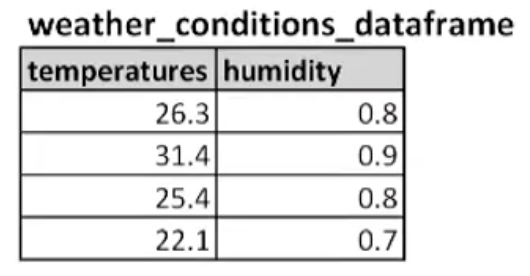
\includegraphics[width=6cm]{dataF1}
\end{center}
\caption{A weather application \texttt{DataFrame}.}
\label{dataF1}
\end{figure}

\item A \texttt{set\_column} method that, given a vector of values of type \texttt{double} and a column name, replaces the entire column content.

In order to complete this task it is better to rely on the following functions:
\begin{itemize}
    \item \texttt{check\_column\_name} checks if a given string is a existing column name in the \texttt{DataFrame};

    \item \texttt{set\_column\_data} stores, given the column name and the column data (i.e., a vector of \texttt{double}), the data in the column.
\end{itemize}

\item A \texttt{get\_column\_names} method, which returns in a \textbf{set} of \texttt{strings} the column names.

\item A \texttt{unique} method, which return the unique values (i.e., without duplicates) stored in the column whose name is passed as parameter.

\item A \texttt{drop\_column} method, which removes from the \texttt{DataFrame} the column whose name is passed as parameters.

\item A \texttt{set\_element\_at} method that, given a column name, an index \texttt{i}, and a value of type \texttt{double}, updates the i-th value of the column.

Try also to implement \texttt{get\_column} and \texttt{get\_element\_at} methods.

\item A \texttt{get\_mean} method, which returns the mean of a given column.

\item A \texttt{sum\_by\_rows} method, which returns in a vector of \texttt{double} the sum of values in each individual row of the \texttt{DataFrame}.

\item A \texttt{select\_equal} method that, given a column name and a value, returns a new \texttt{DataFrame} including only the set of rows for which the column equals the value. For instance,
\texttt{select\_equal ("temperatures", 31.4)} called on the \texttt{DataFrame} in Figure \ref{dataF1} would yield a new one with both columns, but only the second row.

\item A \texttt{concatenate} method, which returns as a copy a \texttt{DataFrame} obtained by concatenating the Dataframe with a second \texttt{DataFrame} passed as parameter (both original \texttt{DataFrame} are left unchanged). An example of concatenation is shown in Figure \ref{dataF2}.
\end{enumerate}

\begin{figure}[h]
\begin{center}
  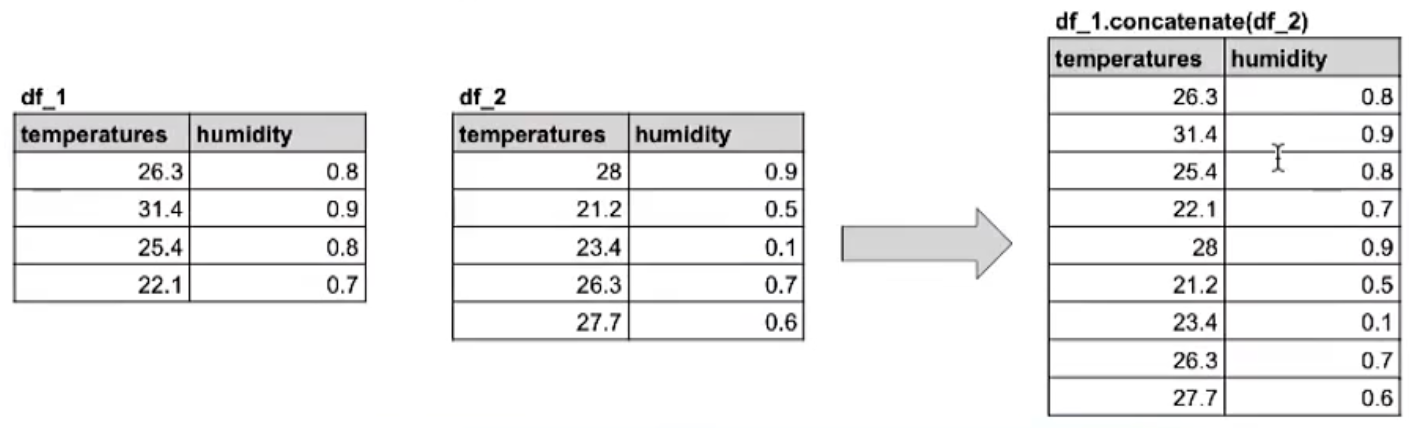
\includegraphics[width=14cm]{dataF2}
\end{center}
\caption{A concatenation of \texttt{DataFrame}s example.}
\label{dataF2}
\end{figure}

Take particular care to error conditions, for example:
\begin{itemize}
    \item access to a wrong column or element index out of range;
    \item check that all the columns have the same number of rows (which will be known only when creating the first column)
\end{itemize}

Finally,
\begin{enumerate}
\setcounter{enumi}{11}
\item Discuss the worst case complexity of the setter methods.
\end{enumerate}


%!TEX root = ../main.tex

\chapter{Evaluate by Column (Exercise 18)}
\thispagestyle{empty}

\begin{table}[H]
    \caption*{\textbf{Header file}}
    \centering 
    \begin{tabular}{ll}
    \hline
    \rowcolor{bluepoli!40} % comment this line to remove the color
    class dense\_matrix final & \\
    \hline
    \textbf{private:} & \\
    & typedef std::vector<double> container\_type \\
    \hline
    \textbf{public:} & \\
    & typedef container\_type::value\_type value\_type \\
    & typedef container\_type::size\_type size\_type \\
    & typedef container\_type::pointer pointer \\
    & typedef container\_type::const\_pointer const\_pointer \\
    & typedef container\_type::reference reference \\
    & typedef container\_type::const\_reference const\_reference \\
    \hline
    \textbf{private:} & \\
    & size\_type m\_rows, m\_columns \\
    & container\_type m\_data \\
    & size\_type sub2ind (size\_type i, size\_type j) const \\
    \hline
    \textbf{public:} & \\
    & dense\_matrix (void) = default \\
    & dense\_matrix (size\_type rows, size\_type columns, const\_reference value = 0.0) \\
    & explicit dense\_matrix (std::istream \&) \\
    & void read (std::istream \&) \\
    & void swap (dense\_matrix \&) \\
    & reference operator () (size\_type i, size\_type j) \\
    & const\_reference operator () (size\_type i, size\_type j) const \\
    & size\_type rows (void) const \\
    & size\_type columns (void) const \\
    & dense\_matrix transposed (void) const \\
    & pointer data (void) \\
    & const\_pointer data (void) const \\
    & void print (std::ostream\& os) const \\
    \hline
    \textbf{outside:} & \\
    & dense\_matrix operator * (dense\_matrix const \&, dense\_matrix const \&) \\
    & void swap (dense\_matrix \&, dense\_matrix \&) \\
    \hline
    \end{tabular}
\end{table}

\newpage

\begin{lstlisting}
  dense_matrix::dense_matrix (size_type rows, size_type columns,
                              const_reference value)
    : m_rows (rows), m_columns (columns),
      m_data (m_rows * m_columns, value) {}

  dense_matrix::dense_matrix (std::istream & in)
  {
    read (in);
  }

  dense_matrix::size_type
  dense_matrix::sub2ind (size_type i, size_type j) const
  {
    return i * m_columns + j;
  }

  void
  dense_matrix::read (std::istream & in)
  {
    std::string line;
    std::getline (in, line);

    std::istringstream first_line (line);
    first_line >> m_rows >> m_columns;
    m_data.resize (m_rows * m_columns);

    for (size_type i = 0; i < m_rows; ++i)
      {
        std::getline (in, line);
        std::istringstream current_line (line);

        for (size_type j = 0; j < m_columns; ++j)
          {
            /* alternative syntax: current_line >> operator () (i, j);
             * or: current_line >> m_data[sub2ind (i, j)];
             */
            current_line >> (*this)(i, j);
          }
      }
  }

  void
  dense_matrix::swap (dense_matrix & rhs)
  {
    using std::swap;
    swap (m_rows, rhs.m_rows);
    swap (m_columns, rhs.m_columns);
    swap (m_data, rhs.m_data);
  }

  dense_matrix::reference
  dense_matrix::operator () (size_type i, size_type j)
  {
    return m_data[sub2ind (i, j)];
  }

  dense_matrix::const_reference
  dense_matrix::operator () (size_type i, size_type j) const
  {
    return m_data[sub2ind (i, j)];
  }

  dense_matrix::size_type
  dense_matrix::rows (void) const
  {
    return m_rows;
  }

  dense_matrix::size_type
  dense_matrix::columns (void) const
  {
    return m_columns;
  }

  dense_matrix
  dense_matrix::transposed (void) const
  {
    dense_matrix At (m_columns, m_rows);

    for (size_type i = 0; i < m_columns; ++i)
      for (size_type j = 0; j < m_rows; ++j)
        At(i, j) = operator () (j, i);

    return At;
  }

  dense_matrix::pointer
  dense_matrix::data (void)
  {
    return m_data.data ();
  }

  dense_matrix::const_pointer
  dense_matrix::data (void) const
  {
    return m_data.data ();
  }

  void 
  dense_matrix::print (std::ostream& os) const
  {
    using size_type = dense_matrix::size_type;

    os << m_rows << " " << m_columns << "\n";
    
    for (size_type i = 0; i < m_rows; ++i)
    {
      for (size_type j = 0; j < m_columns; ++j)
        os << operator () (i,j) << " ";
      os << "\n";
    }
  }

  dense_matrix
  operator * (dense_matrix const & A, dense_matrix const & B)
  {
    using size_type = dense_matrix::size_type;

    dense_matrix C (A.rows (), B.columns ());

    for (size_type i = 0; i < A.rows (); ++i)
      for (size_type j = 0; j < B.columns (); ++j)
        for (size_type k = 0; k < A.columns (); ++k)
          C(i, j) += A(i, k) * B(k, j);

    return C;
  }

  void
  swap (dense_matrix & A, dense_matrix & B)
  {
    A.swap (B);
  }
\end{lstlisting}



















%!TEX root = ../main.tex

\chapter{}
\thispagestyle{empty}

%!TEX root = ../main.tex

\chapter{Lab 01}
\thispagestyle{empty}
%!TEX root = ../main.tex

\chapter{Lab 02}
\thispagestyle{empty}
%!TEX root = ../main.tex

\chapter{Lab 03}
\thispagestyle{empty}
%!TEX root = ../main.tex

\chapter{Lab 04: Iterative solvers and preconditioners with Eigen}
\thispagestyle{empty}

In this lab we aim at evaluating some hand-made implementation of the most common iterative methods for solving linear systems.

\section{Hand-made Conjugate Gradient method}

First, we create a new directory called \texttt{iter\_sol++} and we copy the following implementation of the Conjugate Gradient method in a cpp file called \texttt{eser1.cpp}:

\begin{lstlisting}
namespace LinearAlgebra
{
template <class Matrix, class Vector, class Preconditioner>
int CG(const Matrix &A, Vector &x, const Vector &b, const Preconditioner &M,
   int &max_iter, typename Vector::Scalar &tol)
{
  using Real = typename Matrix::Scalar;
  Real   resid;
  Vector p(b.size());
  Vector z(b.size());
  Vector q(b.size());
  Real   alpha, beta, rho;
  Real   rho_1(0.0);

  Real   normb = b.norm();
  Vector r = b - A * x;

  if(normb == 0.0)
    normb = 1;

  if((resid = r.norm() / normb) <= tol)
    {
      tol = resid;
      max_iter = 0;
      return 0;
    }

  for(int i = 1; i <= max_iter; i++)
    {
      z = M.solve(r);
      rho = r.dot(z);

      if(i == 1)
        p = z;
      else
        {
          beta = rho / rho_1;
          p = z + beta * p;
        }

      q = A * p;
      alpha = rho / p.dot(q);

      x += alpha * p;
      r -= alpha * q;

      if((resid = r.norm() / normb) <= tol)
        {
          tol = resid;
          max_iter = i;
          return 0;
        }

      rho_1 = rho;
    }

  tol = resid;
  return 1;
}
} // namespace LinearAlgebra   
\end{lstlisting}

Hello



\end{document}